\chapter{検定}

\section{概要}

帰無仮説($H_0$)と対立仮説($H_1$)を用意する。
帰無仮説の元での検定量(test statistics)を、実験結果を元に計算する。
その検定量が$H_0$の棄却領域にいれば、帰無仮説を棄却。棄却領域に入らなければ帰無仮説を採択する。
その判定のために、検定量からp-valueを計算して、棄却領域を定義するp-value($\alpha=0.05$)と比較して棄却領域にいるかどうかを検討すればよい。

$H_0$が棄却されるということは、p-valueがしきい値以下であることを示しており、
これは「帰無仮説が現実世界で正しい仮説であると、めったに起こり得ない結果が本実験結果から得られている」とということであり、
それは帰無仮説が正しい、という仮定が間違っていると考えるのが自然であろう。
そのため棄却されるということである。

ここで重要なことは、どんな量を検定量とするかということと、p-valueを計算するために、検定量の従う分布(sampling distribution)の形が既知であることである。
特にその分布を表式できなければならず、方程式は分かるけれどパラメーターが推測できないということはあまり意味がない。
そこでスチューデントのt-検定やカイ二乗検定が出てくるのである。

\section{カイ自乗検定}

\begin{equation}
  \chi^2 = \frac{(x_1-\mu_1)}{\sigma_1^2} + \frac{(x_2-\mu_2)}{\sigma_2^2} + ... + \frac{(x_n-\mu_n)}{\sigma_n^2} = \sum_{i=1}^{n} \frac{(x_i-\mu_i)}{\sigma_i^2}
\end{equation}

カイ自乗の確率関数

\begin{figure}[h]
  \centering
  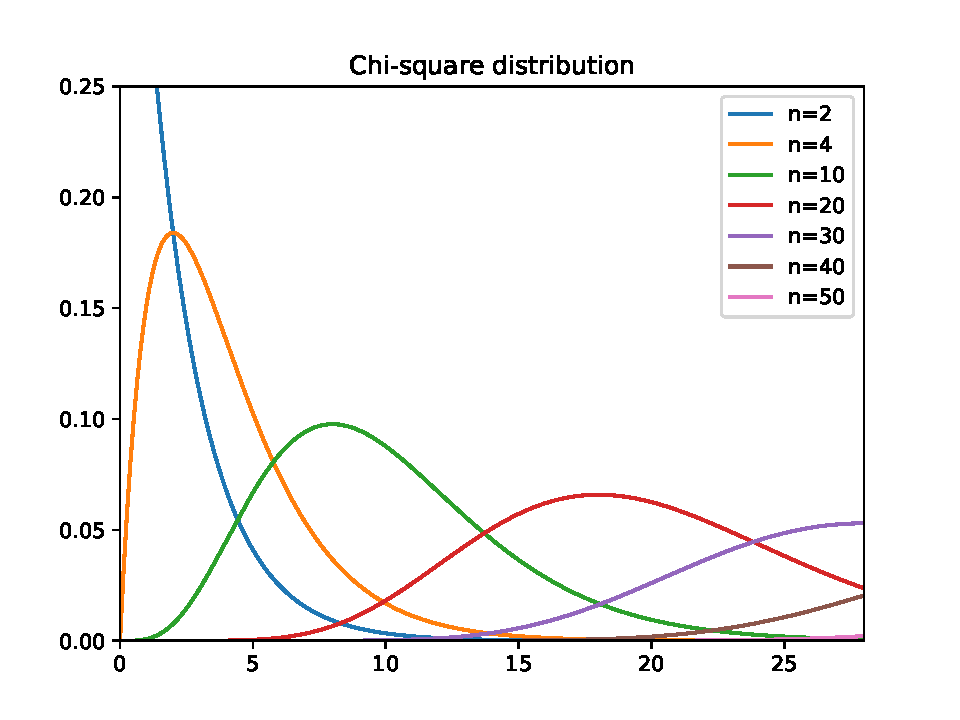
\includegraphics[scale=0.5]{python/ChiSquareDistribution.pdf}
  \caption{$\chi^2$の確率分布。$chi^2$が大きくなるに従って、関数の形が右へシフトしていく。}
\end{figure}


\subsection{どうやってフィットの妥当性を評価するか?}
異なる実験で$Z$ボソンの質量が測定された。これらの実験結果を尤もらしく一つの数値で表現することはできるだろうか?

\begin{table}
  \centering
  \begin{tabular}{lll}
    L3        & $91.161 \pm 0.013$   \\
    OPAL      & $91.174 \pm 0.011$    \\
    Aleph       & $91.186 \pm 0.013$ \\
    Delphi      & $91.188 \pm 0.013$
  \end{tabular}
\end{table}


